\documentclass[12pt]{report}
\usepackage[utf8]{inputenc}
\usepackage[OT1]{fontenc}
\usepackage[francais]{babel}
\usepackage{amsmath}
\usepackage{graphicx}
\usepackage{amsfonts}
\usepackage{amssymb}
\usepackage{enumerate}

\begin{document}
\section{Pince}
La pince doit être à une distance d'un trou de la pièce gris foncé 
(sur le deuxième trou dans la longue barre gris clair). Cette 
distance est en rouge sur la photo. La pièce servant à mettre les 
pièces dans la pince doit être contre la longue barre gris clair.
\begin{center}
		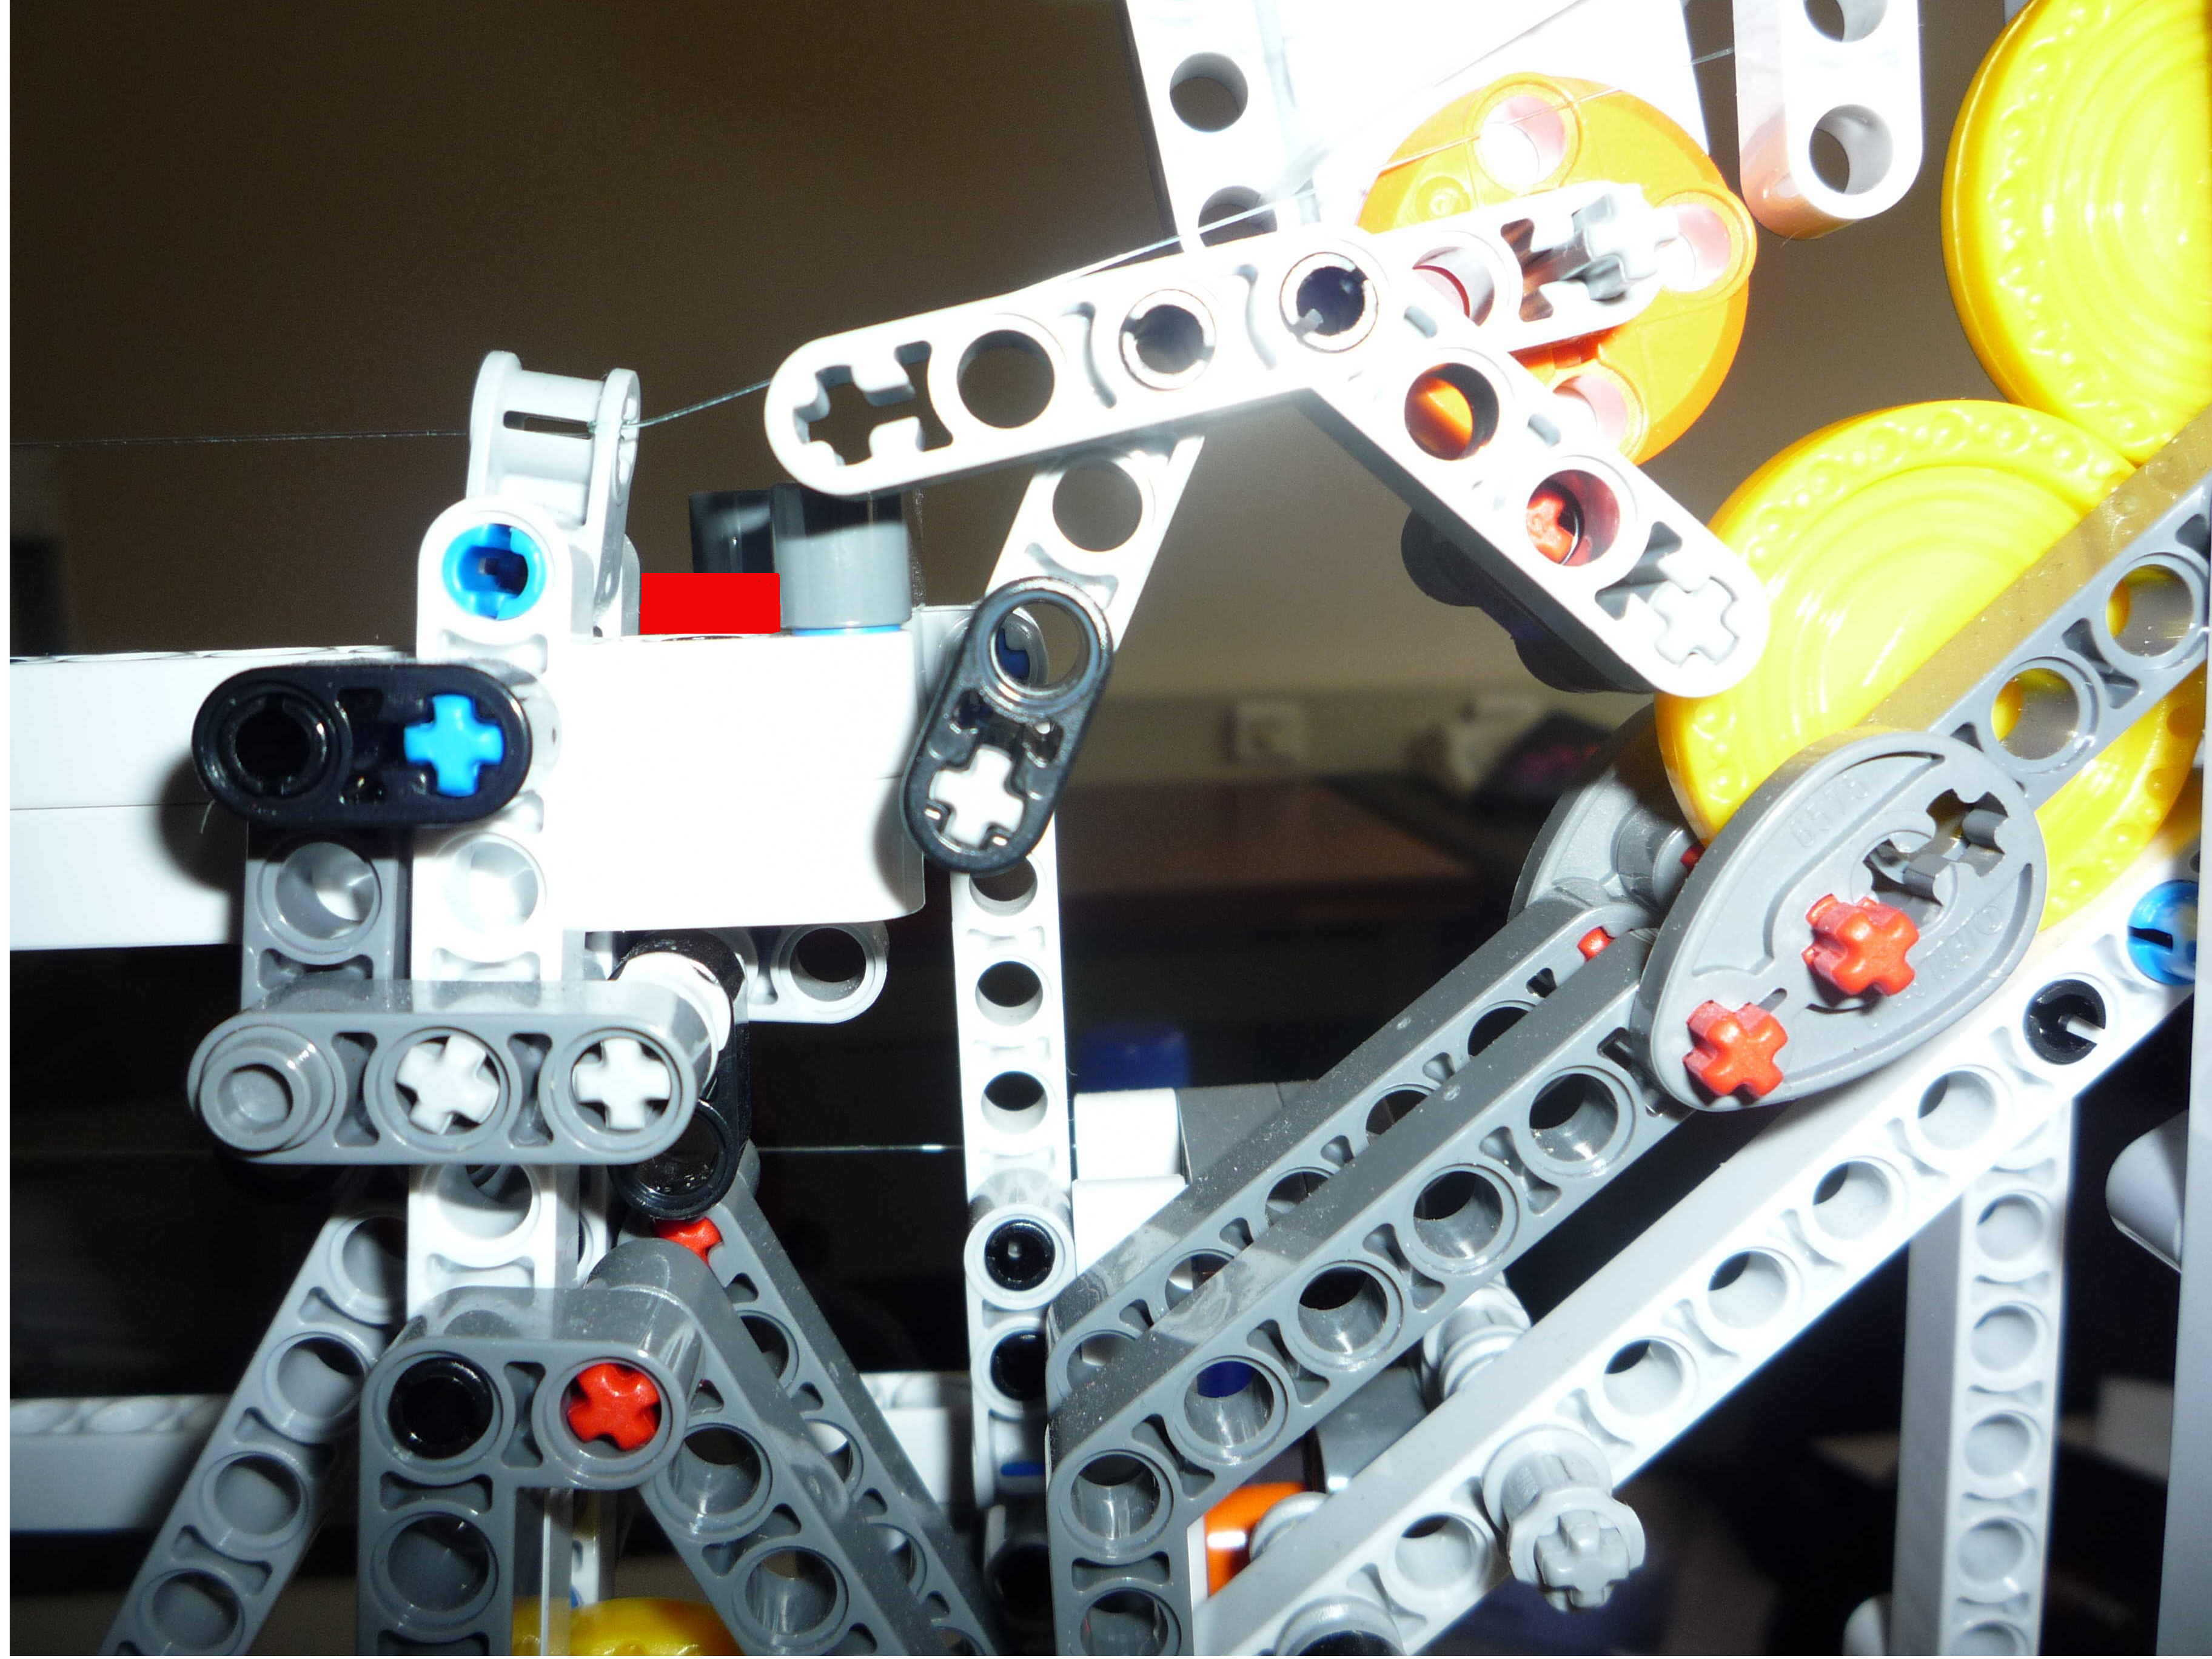
\includegraphics[width=0.7\linewidth]{images/posInitPince.JPG}
\end{center}


Pour le file qui permet d'ouvrir la pince (juste au-dessus du rectangle
rouge sur la photo), celui-ci doit passer juste devant la barre et doit
être tendu mais pas trop, càd on doit pouvoir le baisser très 
légèrement(il doit pouvoir descendre de maximum 2 mm).

\begin{center}
		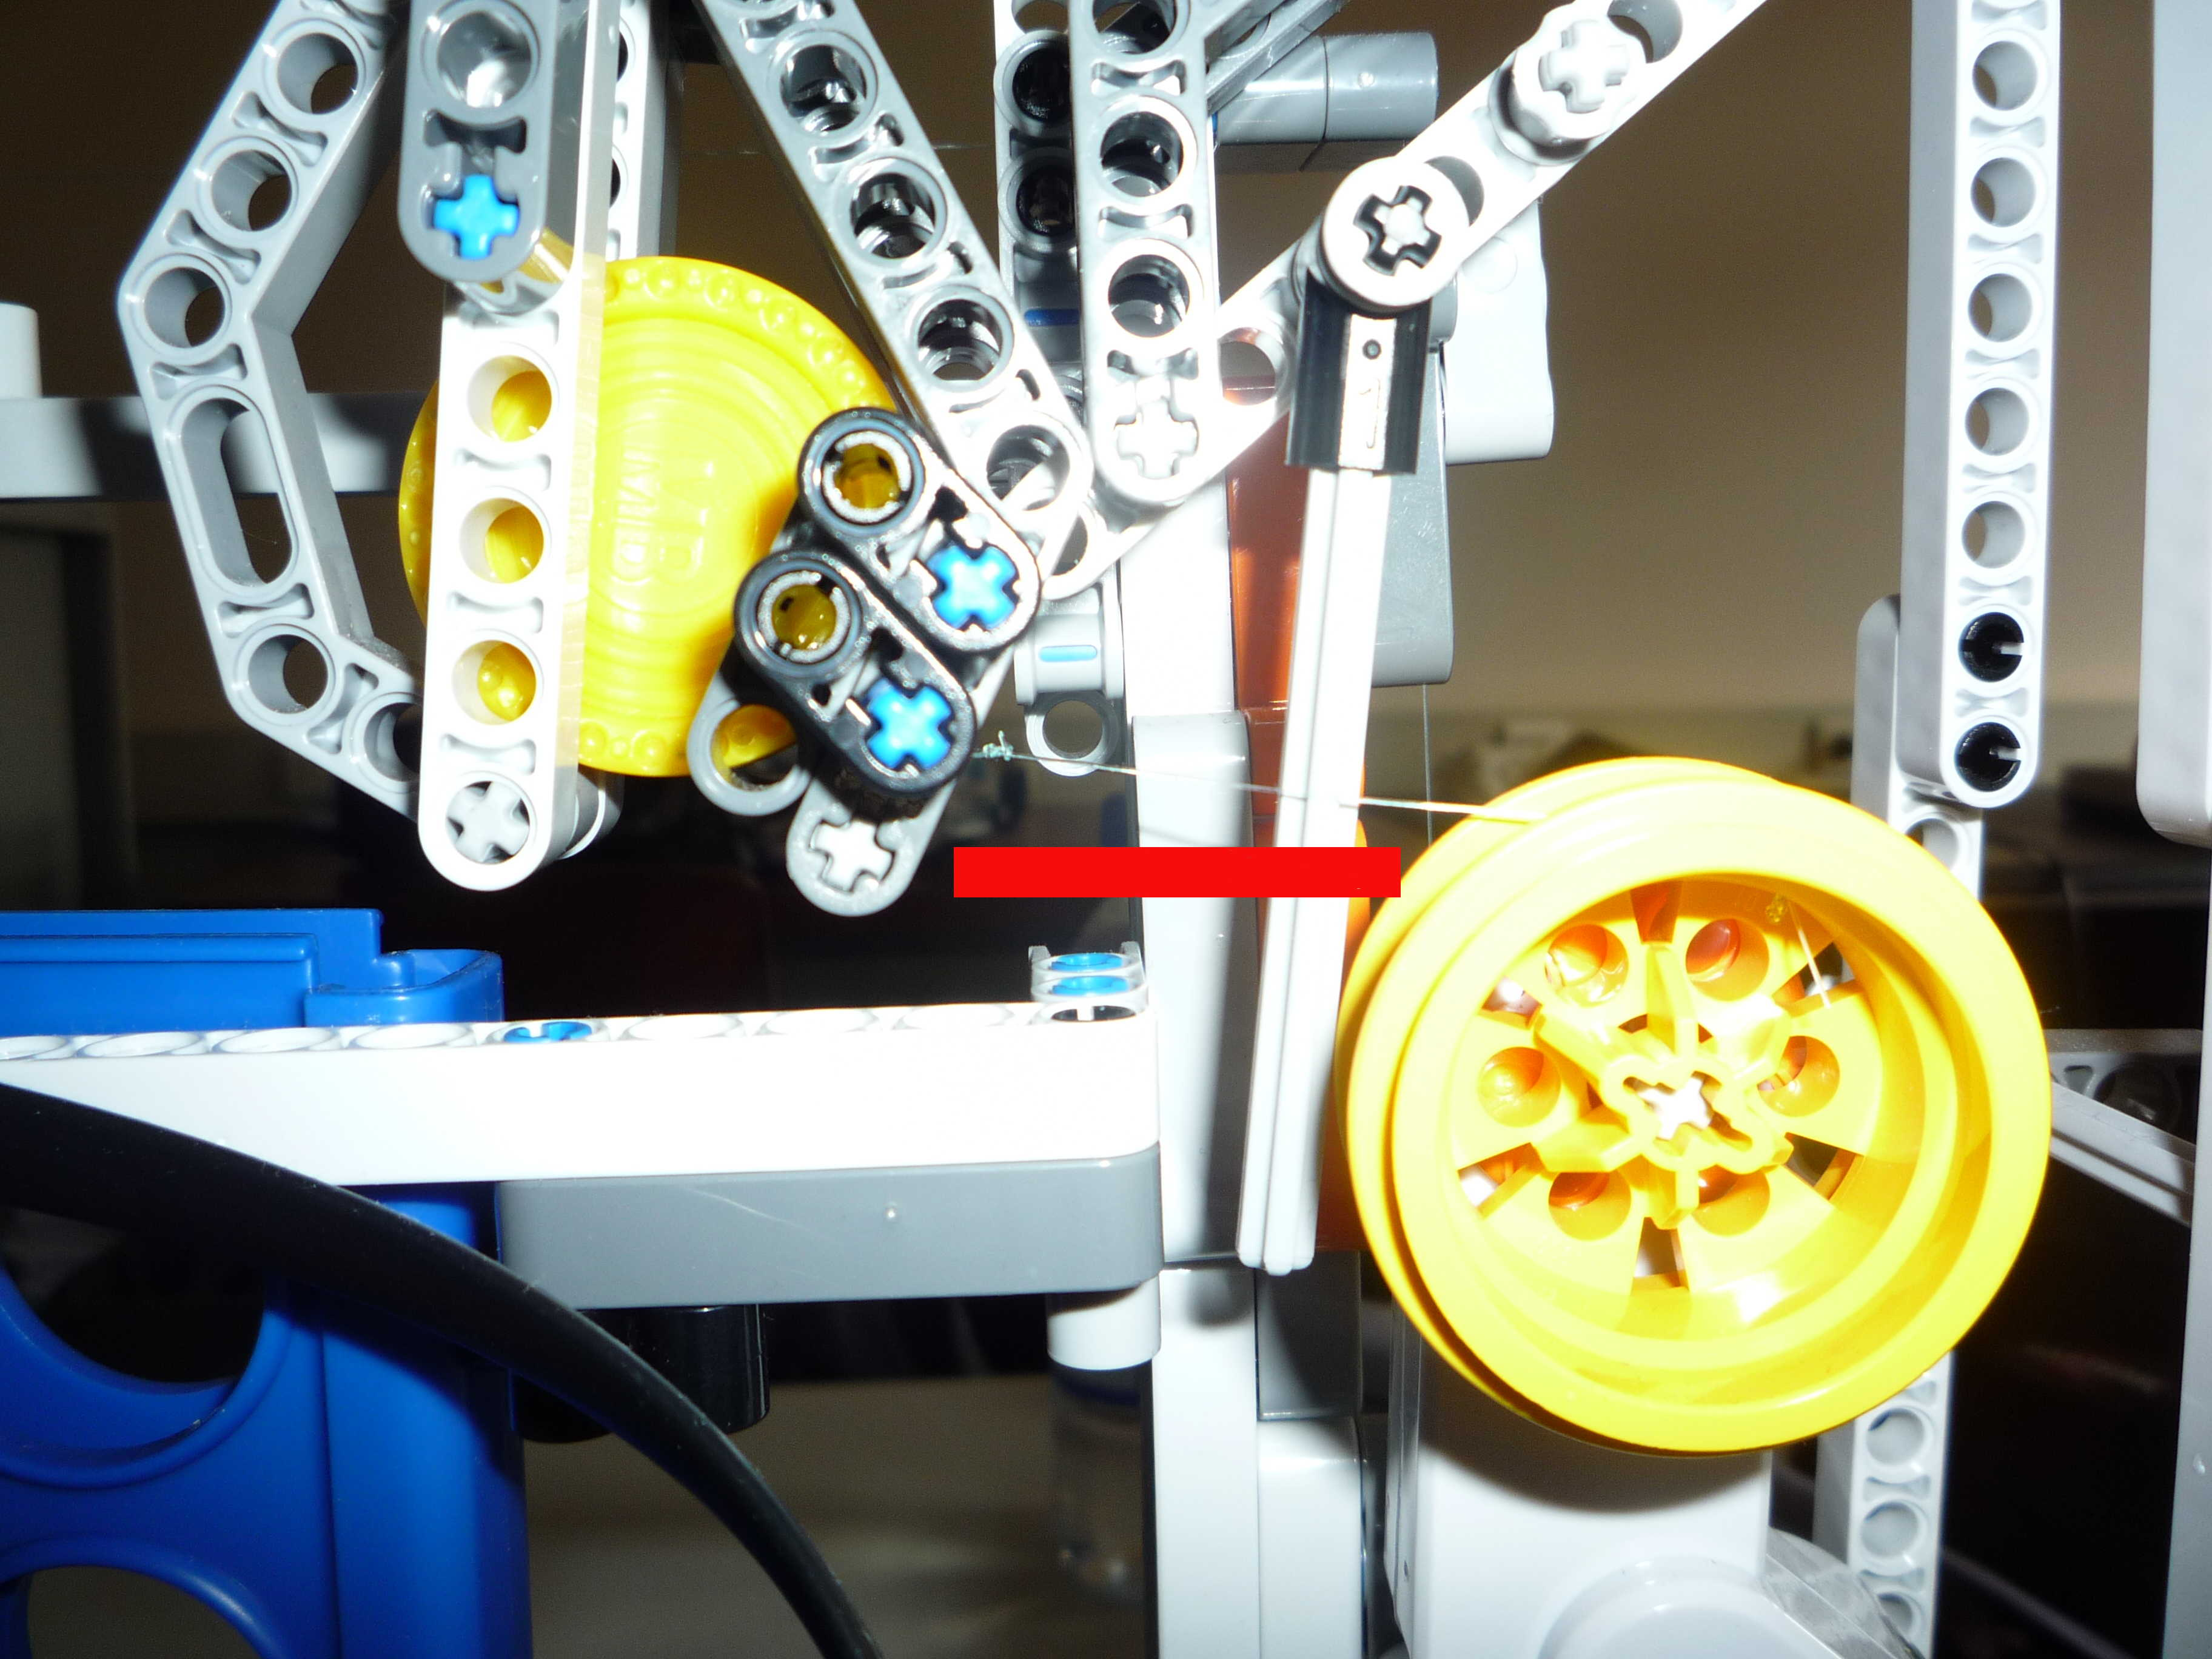
\includegraphics[width=0.7\linewidth]{images/InitFilePince.JPG}
\end{center}

\section{Capteur}
Le capteur doit se trouver du côté opposé au distributeur, il doit être
centré à l'intérieur de la case située tout en bas.

\begin{center}
		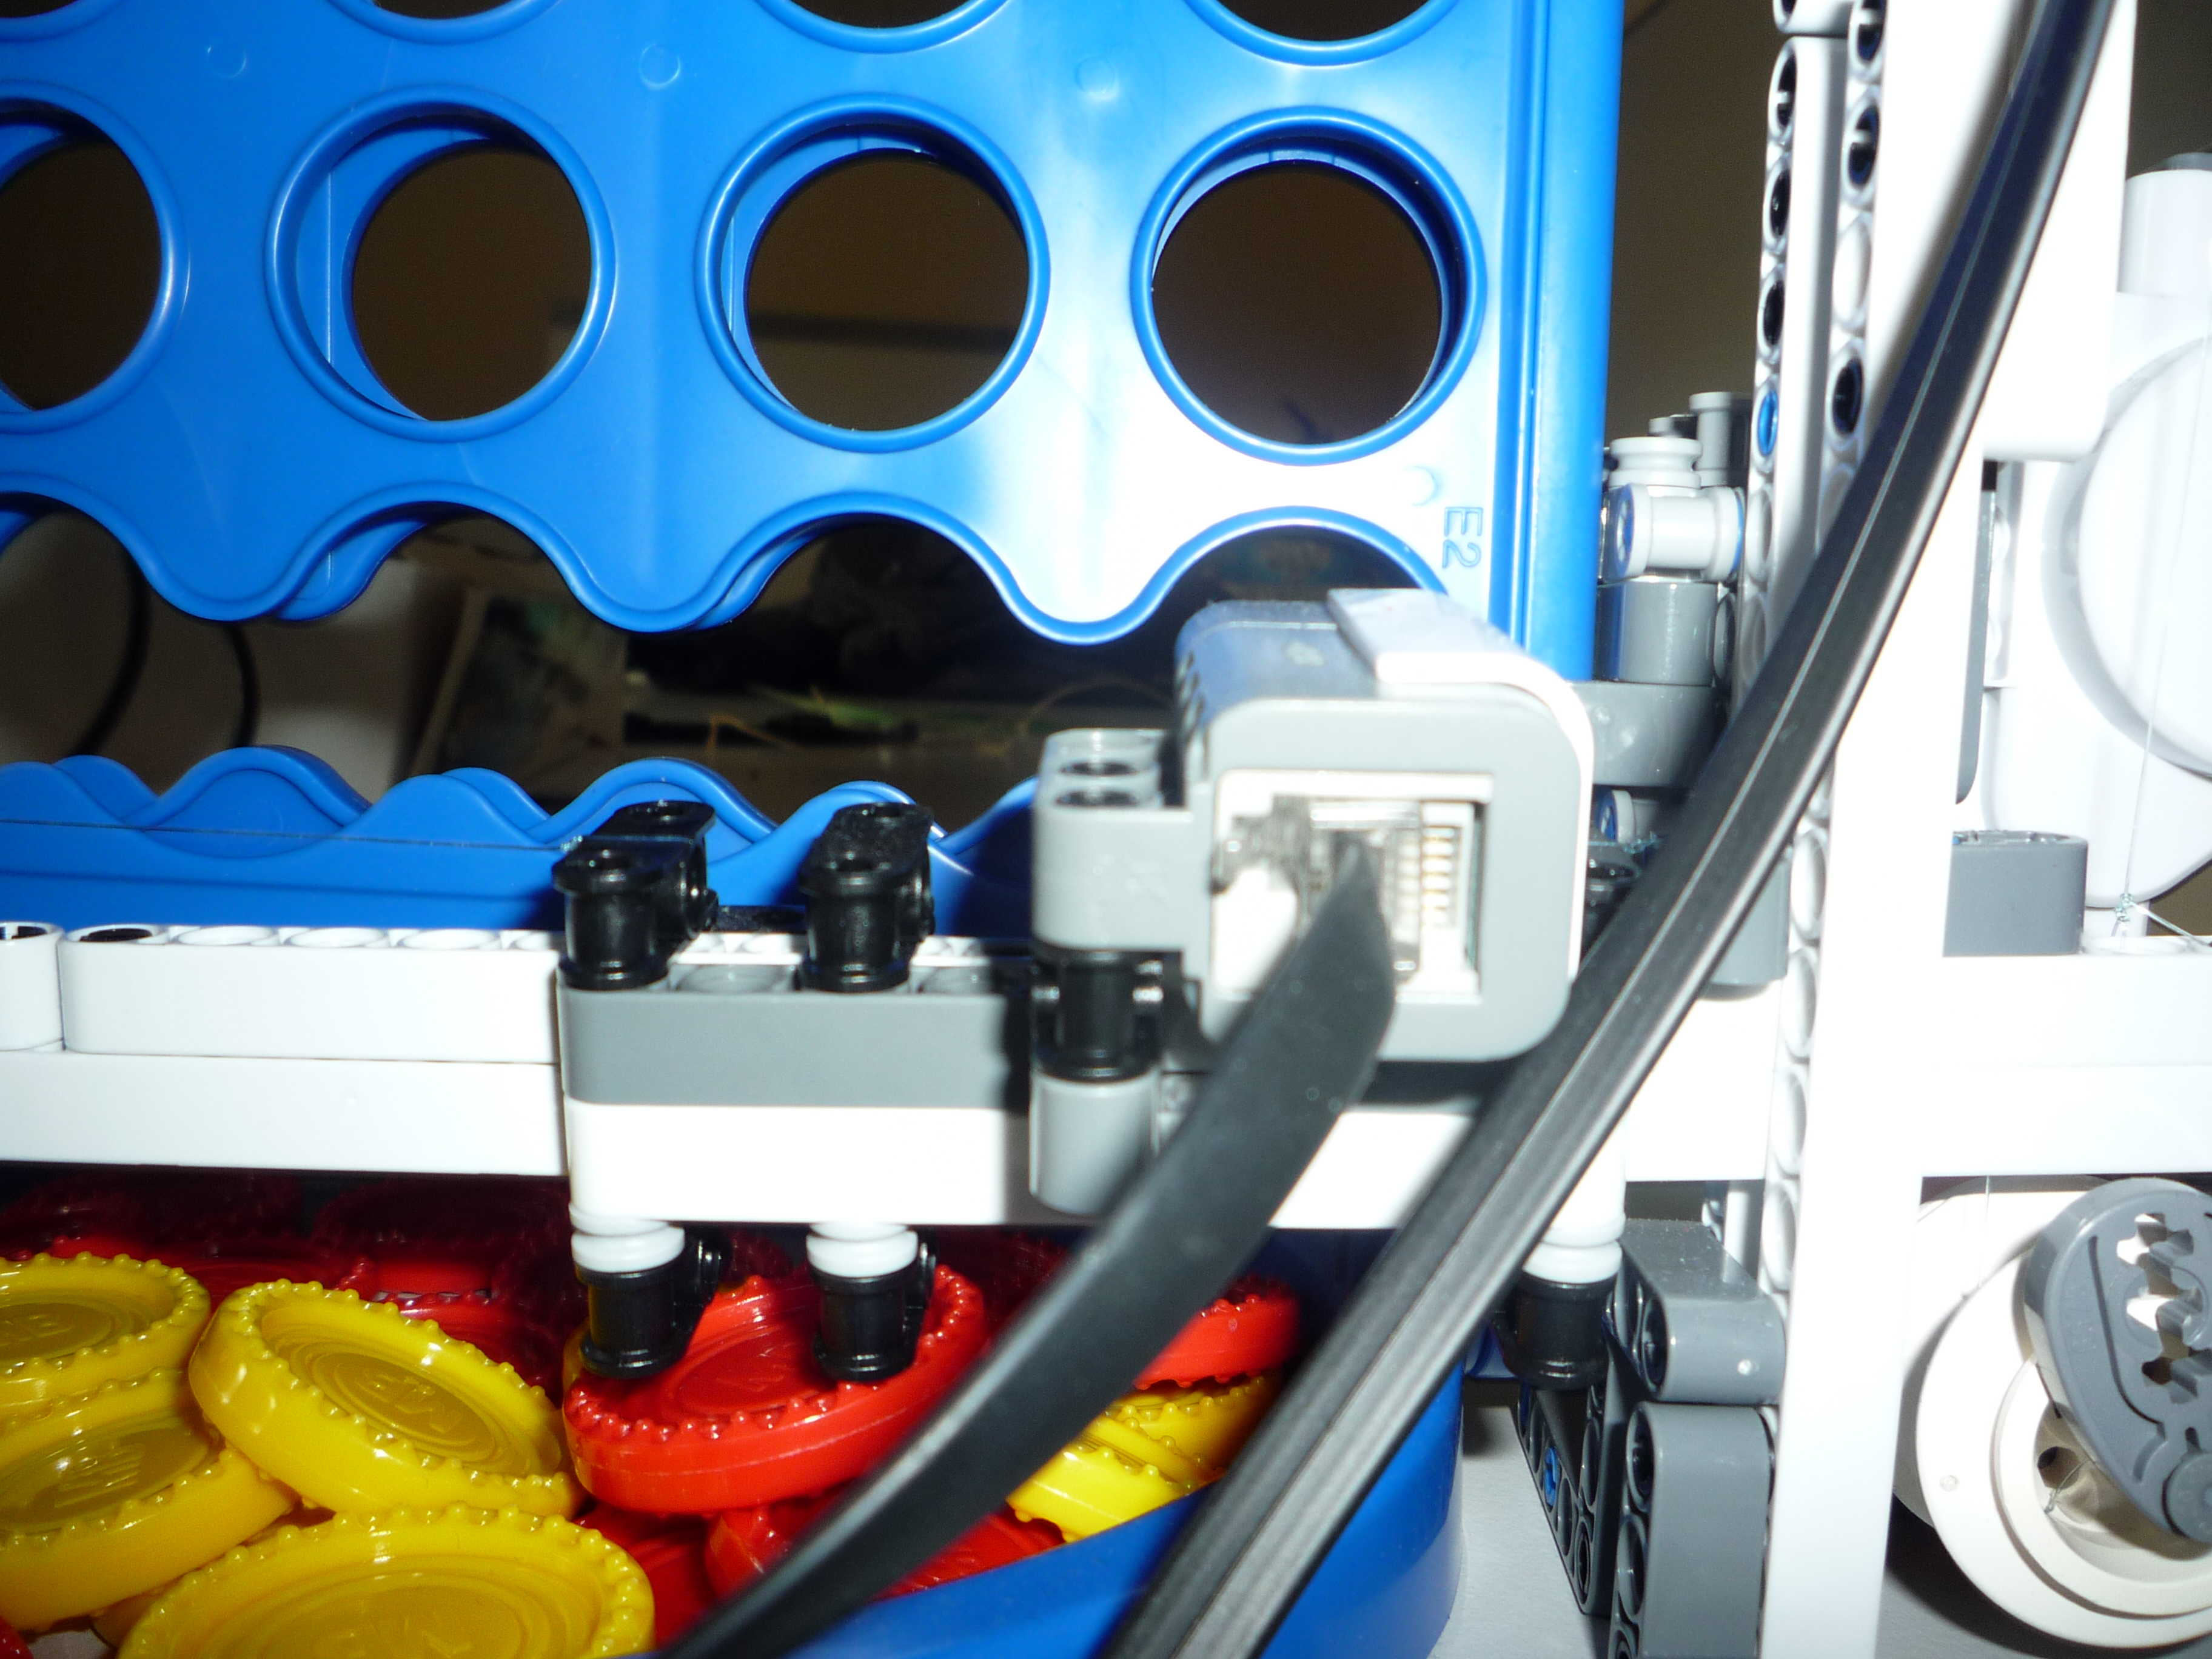
\includegraphics[width=0.7\linewidth]{images/Capteur.JPG}
\end{center}

\begin{center}
	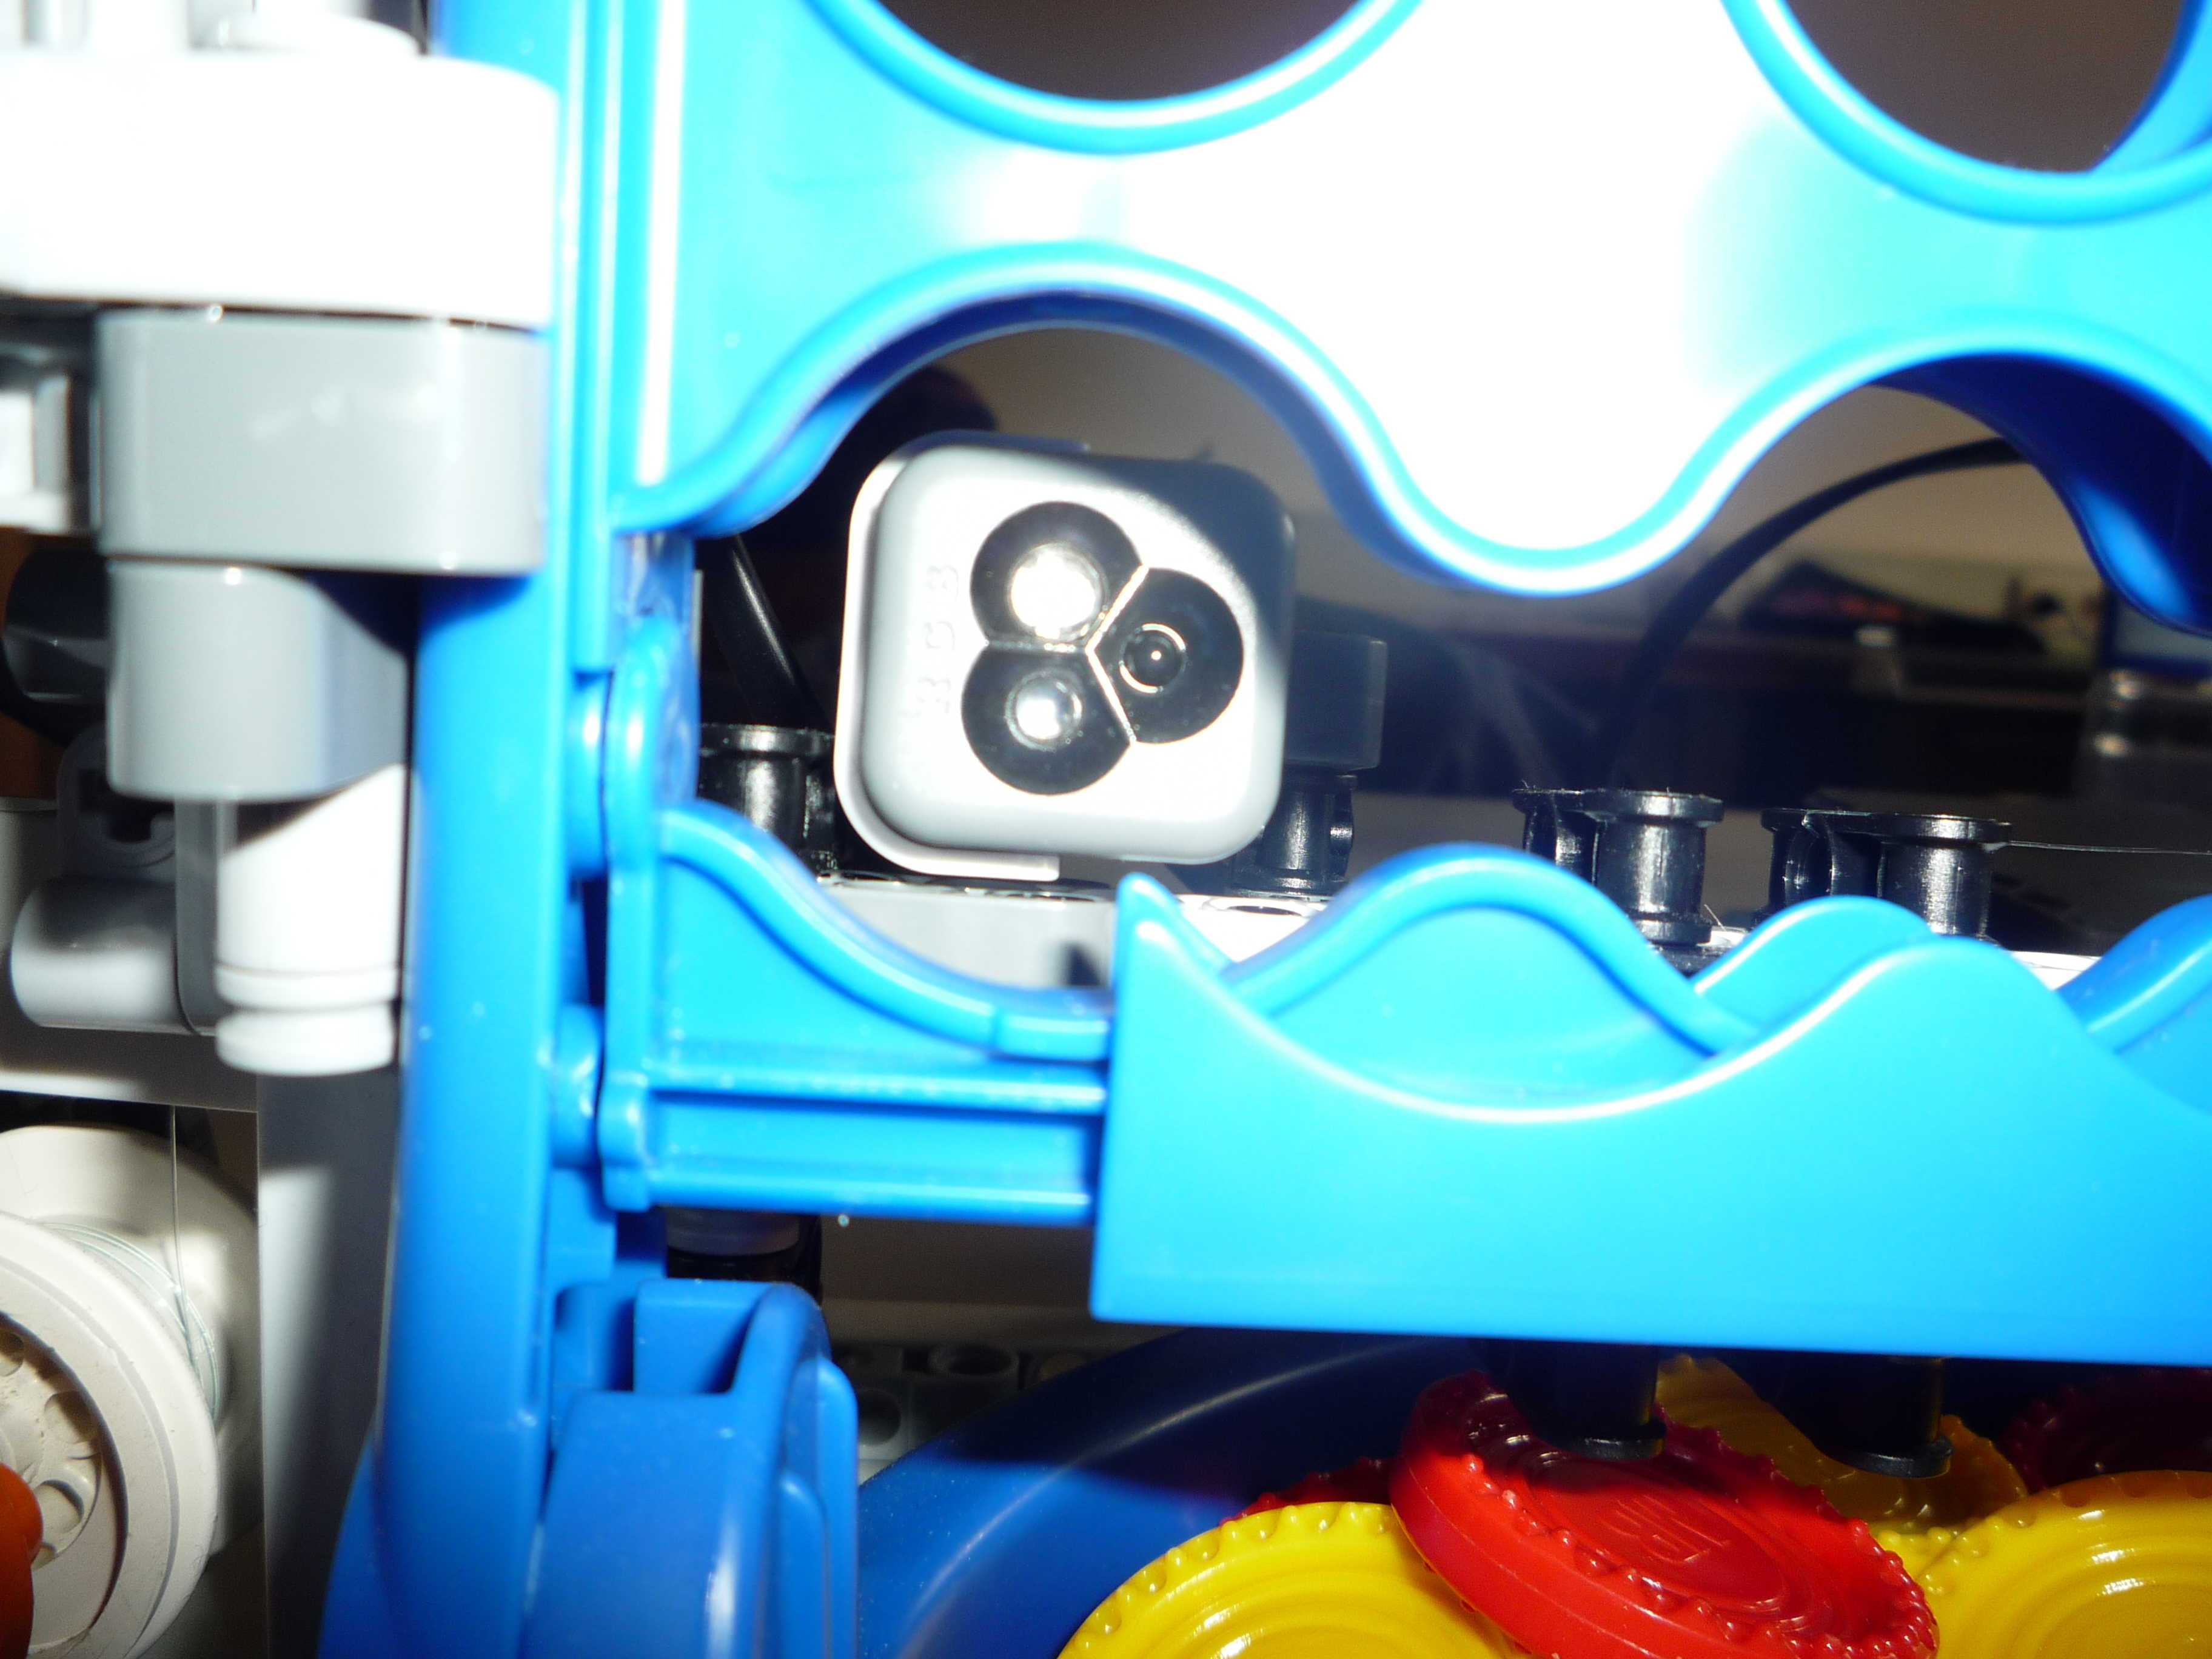
\includegraphics[width=0.7\linewidth]{images/Capteur1.JPG}
\end{center}

\end{document}
